\documentclass{beamer}

\mode<presentation>
{
  \usetheme{CambridgeUS}      % or try Darmstadt, Madrid, ...
  \usecolortheme{default} % or try albatross, beaver, crane, ...
  \usefonttheme{default}  % or try serif, structurebold, ...
  \setbeamertemplate{navigation symbols}{}
  \setbeamertemplate{caption}[numbered]
} 

\usepackage[english]{babel}
\usepackage[utf8x]{inputenc}
\usepackage{listings}
\usepackage[ampersand]{easylist}



\definecolor{KTI_green}{RGB}{150, 189, 13}
\definecolor{TU_red}{RGB}{255, 55, 81}
\definecolor{faint_gray}{RGB}{180, 180, 180}

\definecolor{syntax_green}{rgb}{0,0.6,0}
\definecolor{syntax_gray}{rgb}{0.9, 0.9, 0.9}
\definecolor{syntax_mauve}{rgb}{0.58,0,0.82}

\lstset{ 
  backgroundcolor=\color{syntax_gray},  % choose the background color
  basicstyle=\scriptsize\ttfamily,        		% size of fonts used for the code
  breaklines=false,                		% automatic line breaking only at whitespace
  captionpos=b,                    		% sets the caption-position to bottom
  commentstyle=\color{syntax_green},    % comment style
  escapeinside={\%*}{*)},          		% if you want to add LaTeX within your code
  keywordstyle=\color{blue},       		% keyword style
  stringstyle=\color{syntax_mauve},     % string literal style
  columns=fullflexible,
  frame=single,
  framesep=0.5cm,
  framexleftmargin=0.5cm,
  xleftmargin=0.5cm,
  framexrightmargin=0.5cm,
  xrightmargin=0.5cm,
  frame=tb,                 
    numbers=left,                    
    numbersep=15pt,  
  }
  
  
\newcommand{\logopython}{\raggedleft 
\includegraphics[height=0.5cm]{logo_python}\hspace{0.1cm}\\\raggedright}
\newcommand{\logopythonbottom}{\raggedleft\vspace{-0.8cm}
\includegraphics[height=0.5cm]{logo_python}\hspace*{0.05cm}\\\raggedright}

\title[BSP28 - Monteur]{Monteur}
\author{Dickbauer Y., Moser P., Perner M.}
\institute{PS Computergestützte Modellierung, WS 2016/17}
%\date{Date of Presentation}

\begin{document}

\begin{frame}
  \titlepage
\end{frame}

\begin{frame}{Outline}
  \tableofcontents
\end{frame}

\section{Aufgabenstellung}
\begin{frame}{Aufgabenstellung}
4 gleichartige, unabhängig voneinander operierende Maschinen werden derzeit von einem
Monteur betreut. Die Betriebszeiten jeder Maschine zwischen zwei aufeinanderfolgenden
Ausfällen seien unabhängig und exponentialverteilt mit dem für alle Maschinen gleichen
Parameter $\lambda$ = $\frac{1}{6}$.
\\~\\
Entsprechend seien die Reparaturzeiten der Maschinen unabhängig
voneinander und jeweils exponentialverteilt mit dem Parameter $\mu$ = 1. Fällt eine Maschine
aus, so wird sofort mit ihrer Reparatur begonnen, die von genau einem Monteur
auszufüren ist.
\\~\\
Es wird nun überlegt, einen zweiten Monteur anzustellen.
\end{frame}

\begin{frame}{Aufgabenstellung}
Vergleichen sie die Auslastungen zwischen der Strategie mit einem Monteur und der Strategie
mit zwei Monteuren. Wählen Sie selbst sinnvolle Zahlen für Kosten von Stillstand
und Monteur und bestimmen Sie dadurch die bessere Strategie.
\vspace{1cm}
\begin{itemize}
  \item Eingabe: Feldgröße (Anzahl x, Anzahl y), Ansteckungsrate, optional konfigurierbare Innkubationszeit
  \item Output: Status der Elemente je Periode, Überlebensrate am Ende
\end{itemize}
\end{frame}

\section{Flow Chart}
\begin{frame}{Flow Chart}
	\centering
  	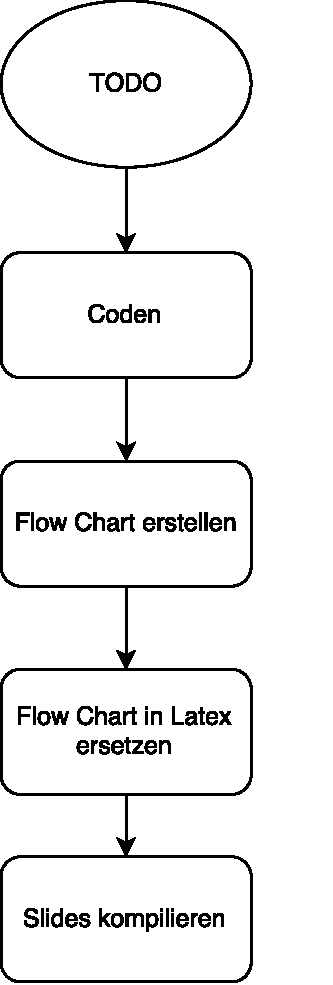
\includegraphics[scale=0.3]{FlowChartTodo.pdf}
\end{frame}

\subsection{Verwendete Funktionen}
%\begin{frame}[fragile]{Funktion loaded\_random\_choice(..)}
  \begin{itemize}
    \item Diese Funktion verlangt eine WSKL Liste als Eingabeparameter
    \item Gibt einen Index zurück, welcher 0 bis $\left\vert{probality\_list}\right\vert-1$ sein kann.
    \item Diese Indizes haben eine gewichtete WSKL, welche jeweils an der Position in der Eingabeliste steht
    \item Beispiel probility\_list := [ 0.9, 0.1 ]  $\Rightarrow$ mit p=90\% wird 0 zurückgegeben, p=10\% für 1
  \end{itemize}
  \begin{lstlisting}[language=python]
def loaded_random_choice(probability_list):
    n = len(probability_list)
    random_number = random.random()
    cum_p = 0
    for i in range(n):
        cum_p += probability_list[i]
        if cum_p > random_number:
            return i
    return None
\end{lstlisting}
\logopythonbottom
\end{frame}	

\section{Grafische Darstellung}

\end{document}
